\chapter{Fourier Analysis}

Fourier analysis is a mathematical tool used to understand and analyze periodic phenomena. It is named after the French mathematician Joseph Fourier, it's based on the idea that any periodic function can be represented as a sum of sine and cosine functions with different frequencies, amplitudes, and phases.

The Fourier transform is one of the most important mathematical tools used for analyzing functions. Given an arbitrary function $f(x)$, with a real domain $(x \in \mathbb{R})$, we can express it as a linear combination of complex waves ($\approx$ change of basis to a frequency domain). 

\begin{itemize}
	\item Periodic Functions: Fourier analysis deals with functions that repeat over regular intervals. This repetition could be over time (like sound waves or electrical signals) or space (like patterns on a surface).
	\item Fourier Series: It states that any periodic function can be represented as an infinite sum of sine and cosine functions. The Fourier series expansion expresses the original function as a weighted sum of sinusoids.
	\item Frequency Domain: While the original function is in the time or spatial domain, Fourier analysis allows us to examine it in the frequency domain. This means we can understand the different frequency components present in the signal and their respective strengths.
	\item Fast Fourier Transform (FFT): This is an efficient algorithm for calculating the Fourier transform of a discrete signal. It's widely used in digital signal processing due to its speed and accuracy.
	\item Continuous vs. Discrete Fourier Transform: While Fourier series deals with periodic continuous functions, Fourier transforms extend the concept to non-periodic functions or signals. The discrete Fourier transform (DFT) is used for discrete, sampled signals, as in digital signal processing.
	\item Inverse Fourier Transform: Just as you can transform a function into the frequency domain using Fourier analysis, you can also transform it back using the inverse Fourier transform. This allows you to reconstruct the original function from its frequency components.
\end{itemize}

\begin{figure}[h]
	\centering
	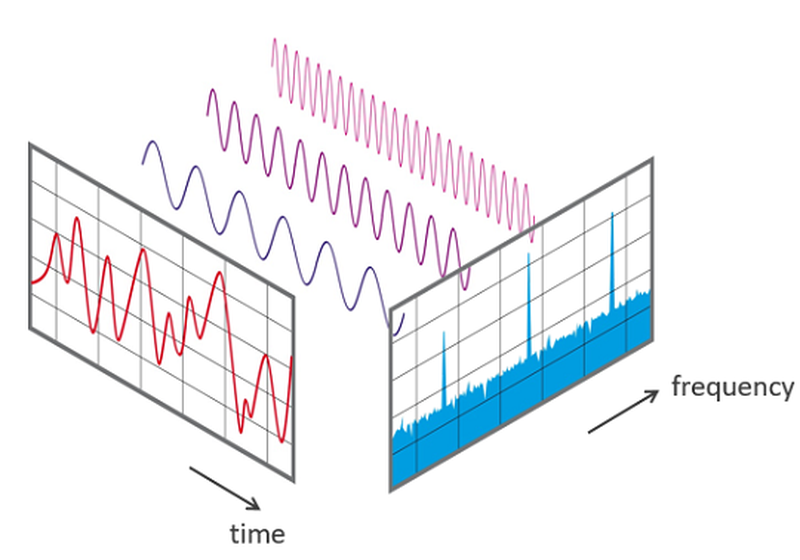
\includegraphics[scale=0.4]{./images/fourier/fourier_intuition.png}
\end{figure}
\textbf{Very intuitive explanation is} \href{https://devincody.github.io/Blog/post/an_intuitive_interpretation_of_the_fourier_transform/}{here!}



\section{Fourier Series}
\label{sec:fourier_series}

We begin by discussing the Fourier series, which is used to analyze functions that are periodic in their inputs. A periodic function $f(x)$ is a function of a real variable $x$ that repeats itself every time $x$ changes by $T$. The constant $T$ is called the \textit{period}. We can write the periodicity condition as
$$f(x+T) = f(x), \forall x\in \mathbb{R}.$$
The value of $f(x)$ can be real or complex, but $x$ should be real.

Let's consider what it means to specify a periodic function $f(x)$. One way to specify the function is to give an explicit mathematical formula for it. Another approach might be to specify the function values in $−T/2 \leq x < T/2$. Since there's an uncountably infinite number of points in this domain, we can generally only achieve an approximate specification of $f$ this way, by giving the values of $f$ at a large but finite set $x$ points. 

There is another interesting approach to specifying $f$. We can express it as a linear combination of simpler periodic functions, consisting of sines and cosines:
\begin{align}
	f(x) = \frac{a_0}{2}+\sum_{n=1}^{\infty} a_n \cos\bigg(\frac{2\pi n x}{T}\bigg)+\sum_{m=1}^{\infty}b_m \sin\bigg(\frac{2\pi m x}{T}\bigg),
	\label{eq:fourier_series}
\end{align}
where $a_0$, $a_n$, and $b_m$ are coefficients determined by integrating $f(x)$ over one period. The coefficients are given by
\begin{align*}
	a_0 &= \frac{1}{T}\int_0^Tf(x)dx\\
	a_n	&= \frac{2}{T}\int_0^Tf(x)\cos\bigg(\frac{2\pi nx}{T}\bigg)dx\\
	b_m	&= \frac{2}{T}\int_0^Tf(x)\sin\bigg(\frac{2\pi nx}{T}\bigg)dx
\end{align*}
The above formula is called a \textit{Fourier series}. Given the numbers $\{a_n, b_m\}$, which are called the \textit{Fourier coefficients}, $f(x)$ can be calculated for any $x$. The Fourier coefficients are real if $f(x)$ is a real function, or complex if $f(x)$ is complex.


\paragraph{Example: }Consider a periodic function $f(x)$ defined on the interval $-\pi\leq x \leq\pi$ as follows:
\begin{align*}
f(x)= 
\begin{cases}
	0 & \text{if } -\pi \leq x < 0 \\
	x & \text{if } 0 \leq x \leq \pi
\end{cases}
\end{align*}

We want to find the Fourier series representation of \( f(x) \).
\paragraph{Solution:} Step 1: Determine the coefficients \( a_0 \), \( a_n \), and \( b_n \).
\begin{enumerate}
	\item Calculate \( a_0 \):
		\begin{align*}
			a_0 &= \frac{1}{\pi} \int_{-\pi}^{\pi} f(x) dx \\
				&= \frac{1}{\pi} \left( \int_{-\pi}^{0} 0 \, dx + \int_{0}^{\pi} x \, dx \right) \\
				&= \frac{1}{\pi} \left( \int_{0}^{\pi} x \, dx \right) \\
				&= \frac{1}{\pi} \left( \frac{1}{2} \pi^2 \right) \\
				&= \frac{\pi}{2} 
		\end{align*}
	\item Calculate \( a_n \): \[ a_n = \frac{1}{\pi} \int_{-\pi}^{\pi} f(x) \cos(nx) \, dx \]
Since \( f(x) \) is odd and \( \cos(nx) \) is even, \( a_n \) will be zero for all \( n \).
	\item Calculate \( b_n \):
		\begin{align*}
			b_n &= \frac{1}{\pi} \int_{-\pi}^{\pi} f(x) \sin(nx) \, dx \\
				&= \frac{1}{\pi} \left( \int_{0}^{\pi} x \sin(nx) \, dx \right) \\
		\end{align*}
		This integral can be evaluated using integration by parts:
\[ u = x, \quad dv = \sin(nx) \, dx \]
\[ du = dx, \quad v = -\frac{1}{n} \cos(nx) \]
\begin{align*}
	b_n &= \frac{1}{\pi} \left( \left[ -\frac{x}{n} \cos(nx) \right]_{0}^{\pi} - \frac{1}{n} \int_{0}^{\pi} -\cos(nx) \, dx \right)\\
		&= \frac{1}{\pi} \left( \frac{\pi}{n} - \frac{1}{n^2} \left[ \sin(nx) \right]_{0}^{\pi} \right)\\
		&= \frac{1}{\pi} \left( \frac{\pi}{n} \right) \\
		&= \frac{1}{n} 
\end{align*}
	\item Write the Fourier series:
\[ f(x) = \frac{\pi}{2} + \sum_{n=1}^{\infty} \frac{1}{n} \sin(nx) \]
\end{enumerate}




\subsection{Square-integrable functions}
Can arbitrary periodic functions always be expressed as a Fourier series? It turns out that a certain class of periodic functions, commonly encountered in physical contexts, are guaranteed to always be expressible as Fourier series. These are called square-integrable functions such that the integral of the square of the absolute value is finite:
\begin{align*}
\int_{-a/2}^{a/2}|f(x)|^2 dx < \infty.
\end{align*}
Unless otherwise stated, we will always assume that the functions we're dealing with are square-integrable.

\subsection{Complex Fourier series and inverse relations}

We have written the Fourier series as a sum of sine and cosine functions. However, sines and cosines can be expressed by exponential functions by using \textit{Euler's formula}. 
\begin{align}
	e^{ix}=\cos x+i\sin x
	\label{eq:euler_formula}
\end{align}
\begin{itemize}
	\item $\cos x=\frac{e^{ix}+e^{-ix}}{2}$
	\item $\sin x=\frac{e^{ix}-e^{-ix}}{2i}$
\end{itemize}
Thus, Fourier series can be expressed as follows:
$$f(x) = \sum_{n=-\infty}^{\infty} c_n e^{inx},$$
where the complex Fourier coefficients \( c_n \) are given by:
\[ c_n = \frac{1}{2\pi} \int_{-\pi}^{\pi} f(x) e^{-inx} \, dx \]

\begin{itemize}
	\item $i$: complex number
	\item $n$: integer
\end{itemize}

\paragraph{Example: }Consider the periodic function \( f(x) \) defined on the interval \( -\pi \leq x \leq \pi \):

\[ f(x) = \begin{cases} 
0 & \text{if } -\pi \leq x < 0 \\
x & \text{if } 0 \leq x \leq \pi 
\end{cases} \]

We will find the complex form of the Fourier series for this function.

#### Step 1: Calculate the complex Fourier coefficients \( c_n \).

\[ c_n = \frac{1}{2\pi} \int_{-\pi}^{\pi} f(x) e^{-inx} \, dx \]

Since \( f(x) \) is piecewise, we split the integral into two parts:

\[ c_n = \frac{1}{2\pi} \left( \int_{-\pi}^{0} 0 \cdot e^{-inx} \, dx + \int_{0}^{\pi} x e^{-inx} \, dx \right) \]

The first integral is zero, so we focus on the second part:

\[ c_n = \frac{1}{2\pi} \int_{0}^{\pi} x e^{-inx} \, dx \]

This integral can be solved using integration by parts. Let:

\[ u = x \quad \text{and} \quad dv = e^{-inx} \, dx \]

Then:

\[ du = dx \quad \text{and} \quad v = \frac{e^{-inx}}{-in} = -\frac{1}{in} e^{-inx} \]

Applying integration by parts:

\[ \int u \, dv = uv - \int v \, du \]

So,

\[ \int_{0}^{\pi} x e^{-inx} \, dx = \left[ -\frac{x}{in} e^{-inx} \right]_{0}^{\pi} + \frac{1}{in} \int_{0}^{\pi} e^{-inx} \, dx \]

Evaluating the boundary terms:

\[ \left[ -\frac{x}{in} e^{-inx} \right]_{0}^{\pi} = -\frac{\pi}{in} e^{-in\pi} - 0 = -\frac{\pi}{in} e^{-in\pi} \]

And for the integral:

\[ \frac{1}{in} \int_{0}^{\pi} e^{-inx} \, dx = \frac{1}{in} \left[ \frac{e^{-inx}}{-in} \right]_{0}^{\pi} = -\frac{1}{n^2} \left( e^{-in\pi} - 1 \right) \]

Combining these results:

\[ \int_{0}^{\pi} x e^{-inx} \, dx = -\frac{\pi}{in} e^{-in\pi} + \frac{1}{n^2} (1 - e^{-in\pi}) \]

Thus, the Fourier coefficient \( c_n \) is:

\[ c_n = \frac{1}{2\pi} \left( -\frac{\pi}{in} e^{-in\pi} + \frac{1}{n^2} (1 - e^{-in\pi}) \right) \]
\[ c_n = \frac{1}{2\pi} \left( -\frac{\pi}{in} (-1)^n + \frac{1}{n^2} (1 - (-1)^n) \right) \]

This expression simplifies to:

\[ c_n = \frac{i(-1)^n}{2n} + \frac{1}{2\pi n^2} (1 - (-1)^n) \]

### Step 2: Write the Complex Fourier Series:

\[ f(x) = \sum_{n=-\infty}^{\infty} c_n e^{inx} \]

With \( c_n \) now calculated, you can substitute these coefficients back into the Fourier series expression to represent \( f(x) \).

\section{Fourier Transform}
\label{sec:fourier_transform}

\subsection{Fourier Series v.s. Fourier Transform}

The Fourier series is used to represent periodic functions as a sum of sine and cosine functions. On the other hand, the Fourier transform extends the idea to non-periodic functions or signals. The Fourier transform of a function \( f(t) \) is given by:
\[ F(\omega) = \int_{-\infty}^{\infty} f(t) e^{-i \omega t} \, dt, \]
where \( F(\omega) \) is the frequency domain representation of the signal \( f(t) \) and $\omega=2\pi f$, where $f$ is a frequency.

\subsection{Equations of Fourier Transform}
The Fourier transform and its inverse are defined as follows:
\begin{itemize}
	\item Fourier Transform:
	\[ F(\omega) = \int_{-\infty}^{\infty} f(t) e^{-i \omega t} \, dt \]
	\item Inverse Fourier Transform:
	\[ f(t) = \frac{1}{2\pi} \int_{-\infty}^{\infty} F(\omega) e^{i \omega t} \, d\omega \]
\end{itemize}
These equations show how a time-domain signal \( f(t) \) can be transformed into its frequency-domain representation \( F(\omega) \), and vice versa.

\paragraph{Example: }The Fourier transform of a rectangular pulse.
Define a rectangular pulse function \( f(t) \) as:
\[ f(t) = \begin{cases} 
1 & \text{if } |t| \leq \frac{1}{2} \\
0 & \text{otherwise} 
\end{cases} \]

To find its Fourier transform \( F(\omega) \):

\[ F(\omega) = \int_{-\infty}^{\infty} f(t) e^{-i \omega t} \, dt \]

Since \( f(t) \) is non-zero only between \( -\frac{1}{2} \) and \( \frac{1}{2} \), the integral becomes:

\[ F(\omega) = \int_{-\frac{1}{2}}^{\frac{1}{2}} e^{-i \omega t} \, dt \]

This integral can be evaluated as:

\[ F(\omega) = \left[ \frac{e^{-i \omega t}}{-i \omega} \right]_{-\frac{1}{2}}^{\frac{1}{2}} = \frac{e^{-i \omega / 2} - e^{i \omega / 2}}{-i \omega} = \frac{2 \sin(\omega / 2)}{\omega} \]

Thus, the Fourier transform of the rectangular pulse is:

\[ F(\omega) = \frac{\sin(\omega / 2)}{\omega / 2} = \text{sinc}\left(\frac{\omega}{2}\right) \]

where \(\text{sinc}(x) = \frac{\sin(x)}{x}\).

\section{Fourier Transform as a Change of Basis}
A change of basis in linear algebra is a fundamental concept that involves transitioning from one coordinate system to another within a vector space. This can simplify calculations, provide deeper insights, or align with different geometric interpretations. Let's break down the concept with definitions and steps:

Fourier analysis is closely related to the concept of change of basis in linear algebra. In Fourier analysis, we are essentially changing the basis from the standard basis of functions (e.g., the time domain for signals) to a basis of sinusoidal functions (\eg the frequency domain). Here’s how this relationship works:

The Fourier transform (both continuous and discrete versions) can be seen as a change of basis from the time domain to the frequency domain. When we apply the Fourier transform to a signal x(t)x(t), we express it as a linear combination of sinusoidal basis functions.

\begin{itemize}
	\item Standard Basis in Time Domain: In the time domain, a signal or function can be represented as a sum of basis functions, which are typically \( \delta \) functions (impulse functions) or other simple functions like polynomial terms. For example, a discrete-time signal \( x[n] \) can be considered in terms of standard basis vectors.

	\item Fourier Basis in Frequency Domain: In the frequency domain, the basis functions are complex exponentials or sinusoidal functions \( e^{i \omega t} \) (where \( i \) is the imaginary unit and \( \omega \) is the angular frequency). The Fourier transform decomposes a signal into a sum of these sinusoidal basis functions.
\end{itemize}

The Fourier transform (both continuous and discrete versions) can be seen as a change of basis from the time domain to the frequency domain. When we apply the Fourier transform to a signal \( x(t) \), we express it as a linear combination of sinusoidal basis functions.

\paragraph{Continuous Fourier Transform:} The continuous Fourier transform of a function \( x(t) \) is given by:
  \[
  X(f) = \int_{-\infty}^{\infty} x(t) e^{-i 2 \pi f t} \, dt
  \]
  Here, \( X(f) \) represents the coordinates of the function \( x(t) \) in the new basis (frequency domain). The inverse Fourier transform reconstructs the original signal from its frequency domain representation:
  \[
  x(t) = \int_{-\infty}^{\infty} X(f) e^{i 2 \pi f t} \, df
  \]
  This process is analogous to converting coordinates from the new basis back to the original basis.

\subsection{Change of Basis}
\begin{itemize}
	\item Vector Space: A collection of vectors where vector addition and scalar multiplication are defined and satisfy specific axioms.
	\item Basis: A set of linearly independent vectors that span the entire vector space. Every vector in the space can be uniquely represented as a linear combination of the basis vectors.
	\item Coordinate Vector: The representation of a vector in terms of the basis vectors, typically given as a column of coefficients.
\end{itemize}

\paragraph{Steps for Change of Basis: }


\begin{enumerate}
	\item Representing Vectors in Original Basis: Given a vector space \( V \) with a basis \( B = \{\mathbf{b}_1, \mathbf{b}_2, \ldots, \mathbf{b}_n\} \), any vector \( \mathbf{v} \) in \( V \) can be written as:
\[ \mathbf{v} = c_1 \mathbf{b}_1 + c_2 \mathbf{b}_2 + \cdots + c_n \mathbf{b}_n \]
Here, \( c_1, c_2, \ldots, c_n \) are the coordinates of \( \mathbf{v} \) relative to basis \( B \), often written as \( [\mathbf{v}]_B \).
	\item Defining the New Basis: Suppose we want to change to a new basis \( B' = \{\mathbf{b}'_1, \mathbf{b}'_2, \ldots, \mathbf{b}'_n\} \). We need to express the original basis vectors in terms of the new basis vectors. Let:
\[ \mathbf{b}_i = a_{i1} \mathbf{b}'_1 + a_{i2} \mathbf{b}'_2 + \cdots + a_{in} \mathbf{b}'_n \]
for \( i = 1, 2, \ldots, n \).
	\item Constructing the Change of Basis Matrix:
The coefficients \( a_{ij} \) form the columns of the change of basis matrix \( P \) from \( B \) to \( B' \):
\[ P = \begin{bmatrix}
a_{11} & a_{12} & \cdots & a_{1n} \\
a_{21} & a_{22} & \cdots & a_{2n} \\
\vdots & \vdots & \ddots & \vdots \\
a_{n1} & a_{n2} & \cdots & a_{nn}
\end{bmatrix} \]
\item Converting Coordinates: To convert the coordinates of a vector \( \mathbf{v} \) from the original basis \( B \) to the new basis \( B' \), we use the change of basis matrix \( P \):
\[ [\mathbf{v}]_{B'} = P^{-1} [\mathbf{v}]_B \]
where \( P^{-1} \) is the inverse of the change of basis matrix and $[\mathbf{v}]_B = (c_1, \dots, c_n)$ is a coordinate vector.
\end{enumerate}

Conversely, to convert coordinates from the new basis \( B' \) back to the original basis \( B \), we use:
\[ [\mathbf{v}]_B = P [\mathbf{v}]_{B'} \]

\paragraph{Example:} Consider a vector space \( \mathbb{R}^2 \) with an original basis \( B = \{\mathbf{b}_1, \mathbf{b}_2\} \) and a new basis \( B' = \{\mathbf{b}'_1, \mathbf{b}'_2\} \). Let:
\[ \mathbf{b}_1 = \begin{bmatrix} 1 \\ 0 \end{bmatrix}, \; \mathbf{b}_2 = \begin{bmatrix} 0 \\ 1 \end{bmatrix} \]
and
\[ \mathbf{b}'_1 = \begin{bmatrix} 1 \\ 1 \end{bmatrix}, \; \mathbf{b}'_2 = \begin{bmatrix} 1 \\ -1 \end{bmatrix} \]

To find the change of basis matrix \( P \) from \( B \) to \( B' \), express the original basis vectors in terms of \( B' \):
\[ \mathbf{b}_1 = \frac{1}{2} \mathbf{b}'_1 + \frac{1}{2} \mathbf{b}'_2 \]
\[ \mathbf{b}_2 = \frac{1}{2} \mathbf{b}'_1 - \frac{1}{2} \mathbf{b}'_2 \]

So, the change of basis matrix \( P \) is:
\[ P = \begin{bmatrix}
\frac{1}{2} & \frac{1}{2} \\
\frac{1}{2} & -\frac{1}{2}
\end{bmatrix} \]

To convert a vector \( \mathbf{v} \) with coordinates \( [\mathbf{v}]_B = \begin{bmatrix} x \\ y \end{bmatrix} \) to the new basis \( B' \), we compute:
\[ [\mathbf{v}]_{B'} = P^{-1} [\mathbf{v}]_B \]

And to revert to the original basis:
\[ [\mathbf{v}]_B = P [\mathbf{v}]_{B'} \]


% ### Practice Problem

% Find the Fourier transform of the function \( f(t) = e^{-a|t|} \) for \( a > 0 \).

% #### Solution Outline

% 1. **Define the function**:
% \[ f(t) = e^{-a|t|} \]

% 2. **Apply the Fourier transform**:
% \[ F(\omega) = \int_{-\infty}^{\infty} e^{-a|t|} e^{-i \omega t} \, dt \]

% 3. **Split the integral**:
% \[ F(\omega) = \int_{-\infty}^{0} e^{at} e^{-i \omega t} \, dt + \int_{0}^{\infty} e^{-at} e^{-i \omega t} \, dt \]

% 4. **Solve each part** and combine the results.

